\documentclass[apacite,jou]{apa6}

\usepackage{amsmath, amssymb, amsthm}
\usepackage[]{natbib}
\usepackage{booktabs}
\usepackage{enumitem}
	\setlist{noitemsep}
	\setlist[description]%
		{font=\normalfont\itshape,%
			 leftmargin=8em, style=multiline} 
	\newenvironment{rdescription}%
		{\begin{description}\raggedright}{\end{description}}
\usepackage[pdfborder={0 0 0}]{hyperref}

\newcommand{\titlesubtitle}[2]{\title{#1\\\vspace{2mm}\large #2}}

\titlesubtitle{Grammar-Based Concept Learning with Numbers and Animals}%
	{9.66 Final Project}
\shorttitle{9.66 Final Project}

\author{Leon Lin}
\affiliation{\mbox{}}

\abstract{\citet{rrdnf} develop a model for concept learning
	through Bayesian inference
	based on the representation of
	 concepts as logical formulae
	generated by a grammar. They show that the model
	explains human performance in learning various artificial
	concepts. In this project we apply largely the same model
	to the domains of numbers and animals. The grammar proves
	to be highly expressive, allowing for an exploration
	of the tradeoff between the complexity of a hypothesis
	and how well it fits the input data.
	 We also compare the model's
	behavior to human intuitions, with mixed results.}

\rightheader{}
\leftheader{}

\newcommand{\Disj}{\text{Disj}}
\newcommand{\Conj}{\text{Conj}}
\newcommand{\True}{\text{True}}
\newcommand{\Prim}{\text{Prim}}
\newcommand{\False}{\text{False}}
\DeclareMathOperator{\diff}{diff}

\begin{document}
\maketitle    
                        
Human minds have a striking ability to learn general concepts from
just a small number of examples. Two or perhaps just one example of,
say, a zebra or a wheel suffices to teach a child those respective
categories.

In this project we build a 
general-purpose Bayesian rule-based concept learner
(\url{https://github.com/leonxlin/concept-learner}) and compare
it to human intuitions in three different domains: numbers, animals,
and a simple artificial domain. 

\section{A grammar for concepts}

In this project we will
model the problem of concept learning much as 
\citet*{rrdnf} do. We provide a 
condensed exposition of their framework, slightly modified to
employ ``strong sampling,'' following one of their suggestions.

Our concept learner lives in a \emph{world}
consisting of a set $W$ of \emph{objects}, each of which may exhibit
some subset of the \emph{features} in the set of possible features.
The learner is aware of exactly which features each object exhibits.

It would be interesting to consider worlds with more structure ---
with nonbinary features or relationships between objects ---
but this setup turns out to be enough for the simple data sets
that we will explore.

A subset~$C\subset W$ of the objects
 belong to a \emph{concept}, which the learner
seeks to learn. A few objects are selected randomly from $C$
(this is strong sampling), and
perhaps a few are also selected from the complement of $C$. These few
objects and an indication of whether each belongs to $C$ are given to
the learner (this is the \emph{observed data}, or input).
 The learner receives
incorrect information about whether a particular object is in $C$ 
with probability $e^{-b}$, for some \emph{outlier parameter} $b$,
as in \citet{rrdnf}.

Given a few positive examples of a concept, there are potentially
many possible larger sets $C$ that contain those examples. How is the
learner to choose from among them? \citet{feldman} found that the most
natural concepts are the simple ones, that is, those with short
representations as boolean propositional formulae in terms of feature
predicates $f_i$, where $f_i(x)$ is true if and only if object $x$
exhibits feature~$i$. Such a formula might look like
\[ x\in C \Leftrightarrow(f_1(x)\wedge f_3(x)) \vee f_2(x).  \]
Again following \citet{rrdnf}, we will consider formulae in
\emph{disjunctive normal form}, such as the one above.
 These formulae are disjunctions
of conjunctions of terms of the form $f_i(x)$ or $\neg f_i(x)$.
A grammar for such formulae is given in 
figure~\ref{dnf1}.\footnote{Actually this grammar generates formulae like
$ x\in C \Leftrightarrow
(f_1(x)\wedge f_3(x)\wedge\True) \vee (f_2(x)\wedge\True)\vee\False$,
which are equivalent.}
\begin{figure}
\begin{align*}
	S &\to x\in C \Leftrightarrow \Disj\\
	\Disj &\to (\Conj) \vee \Disj \\
	\Disj &\to \False \\
	\Conj &\to P \wedge \Conj\\
	\Conj &\to \True\\
	P &\to \Prim\\
	P &\to \neg\Prim\\
	\Prim &\to f_1(x)\\
	\Prim &\to f_2(x)\\
	&\,\,\vdots\\
	\Prim &\to f_N(x)
\end{align*}
	\caption{A modified version
		of the production rules of the
		grammar used in \citet{rrdnf}
		 for formulae in disjunctive normal form
		when there are $N$~features.}
	\label{dnf1}
\end{figure}
With the standard semantics, a formula generated by this grammar
picks out a specific set of objects --- a \emph{hypothesis}
for the concept.

Any partition of the objects into concepts and non-concepts
is specified by some formula, so long as objects with the same 
features are categorized in the same way. Two formulae may define the
same concept.

\section{Prior, likelihood, and posterior}

If the representation of learned concepts in the mind is
something like these formulae, then a rational
learner is interested in the most
likely formulae given the observed data (and the world and the grammar,
which we henceforth assume are always given). Bayes tells us that
for any observed data $D$ and a formula $F$,
\[P(F\mid D) \propto P(F) P(D\mid F). \]

Since we are using strong sampling, the likelihood that we observe $D$,
supposing that $F$ accurately describes the concept,
obeys
\[P(D\mid F) \propto \binom{|C_F|}{|D \cap C_F|}^{-1}
	\binom{|W- C_F|}{|D \cap (W- C_F)|}^{-1}
	e^{-b |\diff(D, F)|}, \]
where $C_F$ is the set of objects belonging to the concept
according to $F$;
$D$, when treated as a set (in a slight abuse of notation),
is the set of objects in the observed data;
and $\diff(D, F)$ is the set of objects that $D$ and $F$ disagree about,
that is, those $x\in D$ for which $D$ says $x\in C$ 
but $F$ says $x\notin C$,
or vice versa.\footnote{We assume $e^{-b} \ll 1$ so that we can ignore
the factors $1-e^{-b}$.}

 To apply
Bayesian inference, we will also need a prior probability distribution
$P(F)$
on the formulae. Remember that we want a prior that penalizes
complicated formulae.

One way to get such a prior is to
assign a probability distribution on the production rules that apply
to each nonterminal symbol in the grammar.
(Thus for instance we might have for the nonterminal symbol $\text{Conj}$
weights of 0.3 and 0.7 on the rules 
	`$\Conj \to P \wedge \Conj$'
and
	`$\Conj \to \True$'
respectively.)
If $\tau$ is a such a set of \emph{production probabilities},
  then the probability $P(F\mid \tau)$ of a
formula~$F$ is the product of the probabilities of each rule used
in its derivation. For example, if there is a uniform probability
distribution on the rules for expanding each nonterminal symbol,
then picking a random formula from the prior is equivalent to
starting with $S$ and picking rules uniformly at random (from 
the applicable ones) until all symbols are terminal. 

To avoid picking a particular set of production probabilities,
we can integrate over them to obtain a prior showing no 
bias to any one of them. \citet{rrdnf} derive this prior. It is
\[P(F) = \prod_Y
	\frac{\beta(\mathbf{C}_Y(F) + \mathbf{1})}{\beta(\mathbf{1})},\]
where $F$ is a formula; the product is over nonterminal symbols $Y$
of the grammar; $\beta$ is the multinomial beta function
\[\beta(c_1,\ldots,c_n) = \frac{\prod_i\Gamma(c_i)}{\Gamma(\sum_i c_i)};\]
$\mathbf{C}_Y(F)$ is a vector  
giving the number of times each production rule
applicable to $Y$ is applied in the unique derivation of $F$ (the order
of the coordinates in the vector doesn't matter); and $\mathbf{1}$ is a
vector of ones having the same length as $\mathbf{C}_Y(F)$, that is,
having as many coordinates as there are rules applicable to $Y$.

\citet{rrdnf} observe that this prior favors not only simple
formulae but also the reuse of rules (and hence 
also the reuse of features predicates
$f_i$). 

The likelihood and the prior enable us to sample from the posterior
$P(F\mid D)$, as is detailed in the next section. We assume
that the learner assesses the probability that some object $x$
is in $C$
(the \emph{generalization probability})
 by consulting a few likely hypotheses drawn from
the posterior (and weighting their judgments of $x$ according 
to their respective posterior probabilities). \citet{rrdnf}
defend this choice --- \emph{hypothesis sampling} --- but do not
say exactly how many hypotheses (formulae) should be considered.
The number $\phi$ of formulae to take from the
top of the list may be used as another
free parameter (along with $b$), but in this project 
we will always take $\phi=10$.


\section{Method}

Given $D$
we sample from the posterior distribution on formulae
 using the Metropolis-Hastings
algorithm. Code implementing this algorithm is available at
\url{https://github.com/leonxlin/concept-learner}.

We use the same Markov chain on formulae as \citet{rrdnf} do.
Given a formula $F$, a proposal formula $F'$ is chosen by
randomly selecting a nonterminal node of $F$ and regenerating its
subtree in the unique parse tree of $F$ using a uniform set $\tau$ of
production probabilities as described above.
If $F=F'$ the process is repeated. Let $Q(F' \mid F)$ be the 
probability that a particular $F'$ is proposed given $F$.
With a counting argument one can show that
\[ \frac{Q(F\mid F')}{Q(F'\mid F)}
	 = \frac{|F|\,P(F\mid\tau)}{|F'|\,P(F'\mid\tau)}, \]
where $|F|$ is the number of nonterminal nodes in the parse tree
of $F$. Then accepting 
(transitioning from $F$ to)
$F'$ with probability equal to the minimum of $1$ and
\begin{align*}
	\frac{P(F'\mid D)}{P(F\mid D)}\cdot
	\frac{Q(F\mid F')}{Q(F'\mid F)} = 
	\frac{P(D\mid F')P(F')}{P(D\mid F)P(F)}\cdot
	\frac{|F|\,P(F\mid\tau)}{|F'|\,P(F'\mid\tau)}
\end{align*}
makes the Markov chain converge to the posterior distribution
$P(F\mid D)$.


\section{A four-feature world}

As a sanity check we apply the model to a certain world of objects
proposed by \citet{medin}
and compare it to responses from humans 
gathered by \citet{nosofsky},
 though they
do not assume strong sampling.

\begin{figure}
\centering
\begin{tabular*}{\columnwidth}{@{\extracolsep{\fill} } ccccc}
	\toprule
	Object & Features & Human & Model, $b=1.3$ & $b=5$ \\ \midrule
	A1 & 0001 & 0.77 & 0.79 & 1.00 \\
	A2 & 0101 & 0.78 & 0.79 & 1.00 \\
	A3 & 0100 & 0.83 & 0.87 & 1.00 \\
	A4 & 0010 & 0.64 & 0.57 & 1.00 \\
	A5 & 1000 & 0.61 & 0.54 & 0.95 \\\midrule
	B1 & 0011 & 0.39 & 0.49 & 0.05 \\
	B2 & 1001 & 0.41 & 0.46 & 0.00 \\
	B3 & 1110 & 0.21 & 0.26 & 0.00 \\
	B4 & 1111 & 0.15 & 0.18 & 0.00 \\ \midrule
	T1 & 0110 & 0.56 & 0.57 & 0.13 \\
	T2 & 0111 & 0.41 & 0.49 & 0.05 \\
	T3 & 0000 & 0.82 & 0.87 & 1.00 \\
	T4 & 1101 & 0.40 & 0.46 & 0.00 \\
	T5 & 1010 & 0.32 & 0.26 & 0.87 \\
	T6 & 1100 & 0.53 & 0.54 & 0.08 \\
	T7 & 1011 & 0.20 & 0.18 & 0.00 \\\bottomrule
\end{tabular*}
\bigskip\mbox{}
\caption{Objects and features in a world proposed by \citet{medin},
	with human data
	(recognition rates) from \citet{nosofsky} and the
	generalization probabilities of our model.
	There are four possible features, and the features each
	object exhibits are indicated with binary strings (1 for yes
	and 0 for no). The objects A1--A5 are observed to be
	examples of the concept; the objects B1--B4 are observed
	to not be examples of the concept.}
\label{medindata}
\end{figure}

The world consists of 16 objects, exhibiting all possible
subsets of four features. Five of the objects are given as
positive examples of a concept; four are given as negative
examples.

The results 
of 30000 samples with $b=1.3$
and 30000 samples with $b=5$ are shown in figure \ref{medindata}.
The fit between our model with $b=1.3$ and the human data
 was $R^2 = 0.95$.
The top $\phi=10$ formulas sampled with $b=1.3$ were as follows.
\begin{enumerate}
	\item $x\in C\Leftrightarrow 
		(\neg f_1(x)\wedge\True)\vee\False$
	\item $x\in C\Leftrightarrow 
		(\neg f_3(x)\wedge\True)\vee\False$
	\item $x\in C\Leftrightarrow 
		\False$
	\item $x\in C\Leftrightarrow 
		(\True)\vee\False$
	\item $x\in C\Leftrightarrow 
		(\neg f_4(x)\wedge\True)\vee\False$
	\item $x\in C\Leftrightarrow 
		(\neg f_1(x)\wedge\neg f_1(x)\wedge\True)\vee\False$
	\item $x\in C\Leftrightarrow 
		(\True)\vee(\True)\vee\False$
	\item $x\in C\Leftrightarrow 
		(\neg f_3(x)\wedge\neg f_3(x)\wedge\True)\vee\False$
	\item $x\in C\Leftrightarrow 
		(\True)\vee(\True)\vee(\True)\vee\False$
	\item $x\in C\Leftrightarrow 
		(\neg f_1(x)\wedge\neg f_3(x)\wedge\True)\vee\False$
\end{enumerate}
The low outlier parameter, i.e., high tolerance for error in the
observed data, combined with the prior's bias toward simple
formulas allows such formulae as `$\False$' and `$(\True)\vee\False$'
to make the top ten.
The nature of our grammar allows a high degree of redundancy 
both between and within formulae. Though the plausibility
of some of these formulae as mental representations of concepts
is dubious, the model seems to correlate well with human behavior.

With $b=5$, the balance between fit and rule complexity tips toward
the former, and for most of the top ten formulas 
the condition on $x\in C$ was a variation on
\[ (\neg f_1(x)\wedge\neg f_3(x)\wedge\True) \vee
	(\neg f_2(x)\wedge\neg f_4(x)\wedge\True) \vee\False. \]


\section{A world of numbers}

\citet{numbergame} found that a Bayesian model predicted human
learning of categories of integers from 1 to 100. The model's
hypothesis space included categories of multiples such as
$\{2,4,\ldots,100\}$ and $\{9, 18,\ldots,99\}$ and categories of 
consecutive numbers of such as $\{33,34,\ldots,41\}$, among other
possible categories.

Accordingly we consider the following set of 62 features:
for $i=2,\ldots,30$ let $f_i(x)$ be true when $x$ is a multiple of $i$
and for $i=3,6,\ldots,99$ 
let $g_i(x)$ be true when $|x-i| \leq 5$.
(These particular values of $i$ are not special; they are chosen
so that the total number of features is manageable.)
These features, together with our grammar, allow us to express
a wide variety of concepts, such as `multiples of 3' and
`multiples of 20 and odd numbers greater than 90.' 

\begin{figure}
\begin{align*}
	S &\to x\in C \Leftrightarrow \Disj\\
	\Disj &\to (\Conj) \vee \Disj \\
	\Disj &\to \Conj \\
	\Conj &\to P \wedge \Conj\\
	\Conj &\to P\\
	P &\to \Prim\\
	P &\to \neg\Prim\\
	\Prim &\to \True\\
	\Prim &\to f_1(x)\\
	\Prim &\to f_2(x)\\
	&\,\,\vdots\\
	\Prim &\to f_N(x)
\end{align*}
	\caption{A modified version of our grammar, designed to 
		reduce the weight of formulas equivalent to $\True$
		or $\False$ in the prior.}
	\label{dnf2}
\end{figure}

Sampling formulae from the posterior with various observed data
(e.g., $\{62, 52, 57, 55\}$), we find that the most likely
formulae are mostly equivalent to `$\True$'. This happens because 
in the grammar,
the large number of features causes any particular
nontrivial conjunction
to be quite unlikely in the prior, which causes the posterior to 
strongly favor formulae that don't involve any features.
 Therefore we will use
the modified grammar in figure~\ref{dnf2}, which induces
a prior much less heavily weighted toward formulae like
`$(\True)\vee(\True)\vee\False$'.

\begin{figure*}
    \newcommand{\Scale}{0.42}
    
    \noindent
    \begin{tabular}{@{}p{0.5\textwidth}@{}p{0.5\textwidth}@{}}
    Observed: $60\in C$ & Observed: $\{60, 80, 10, 30\} \subset C$ \\
	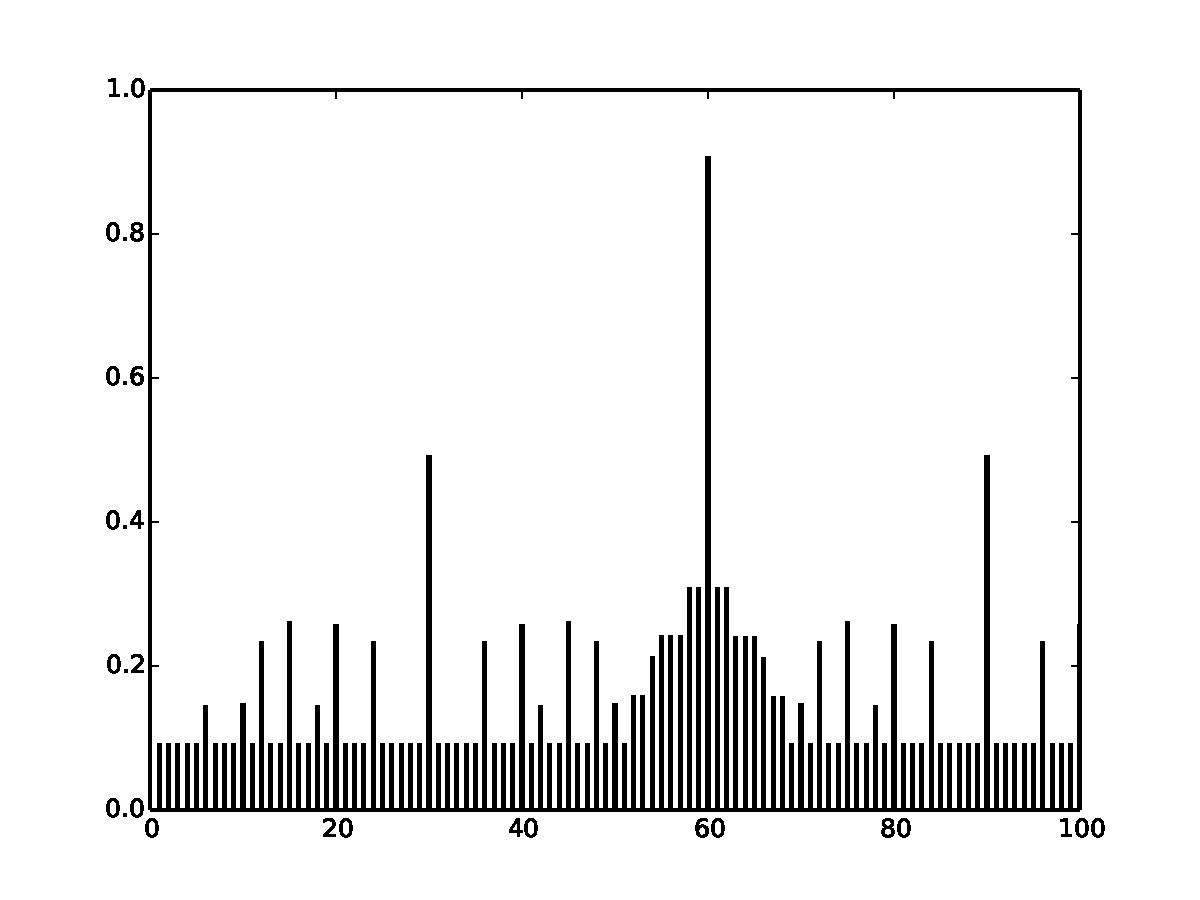
\includegraphics[scale=\Scale]{ng60.pdf} &
	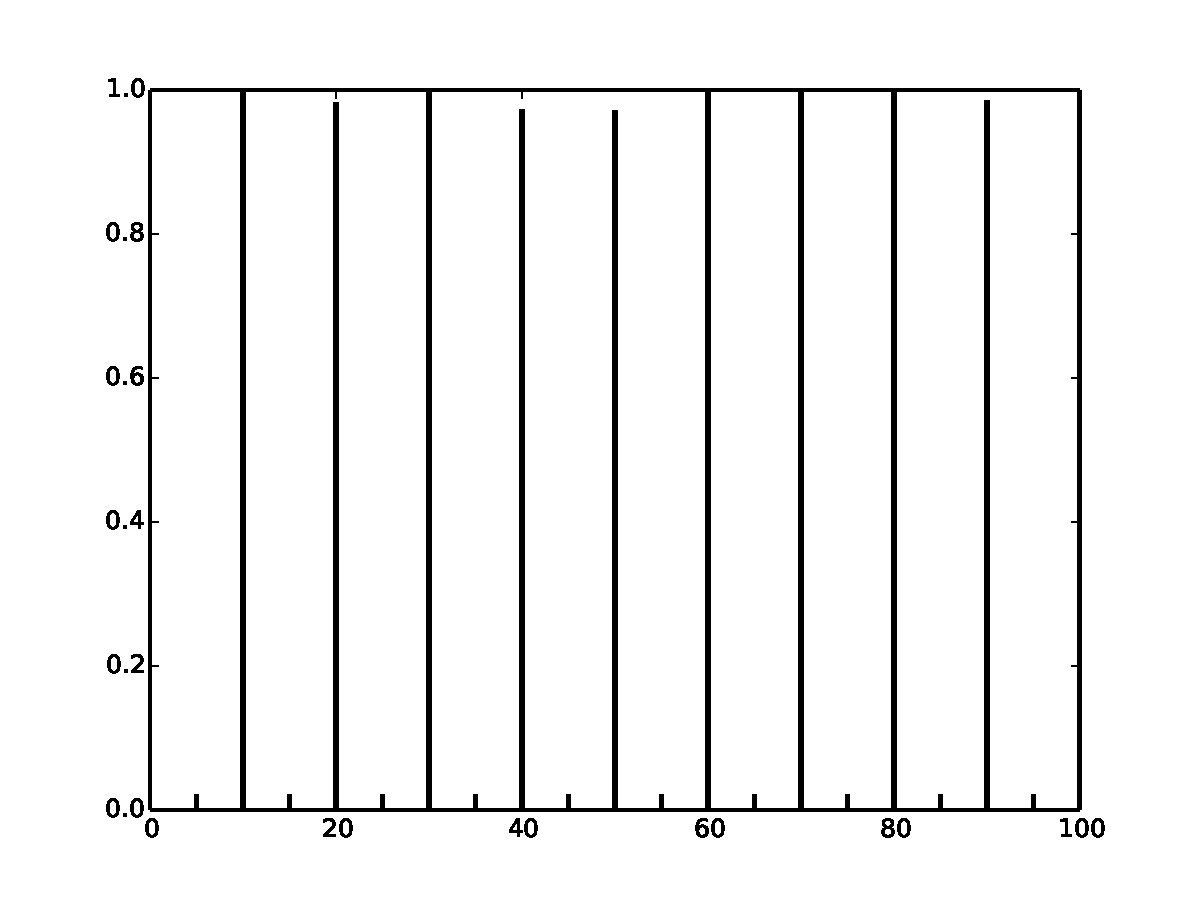
\includegraphics[scale=\Scale]{ng60801030.pdf}\\[2em]
	Observed: $\{60, 80, 10, 30, 23\} \subset C$ &
	Observed: $\{60, 80, 10, 30, 23, 25, 21\} \subset C$ \\
	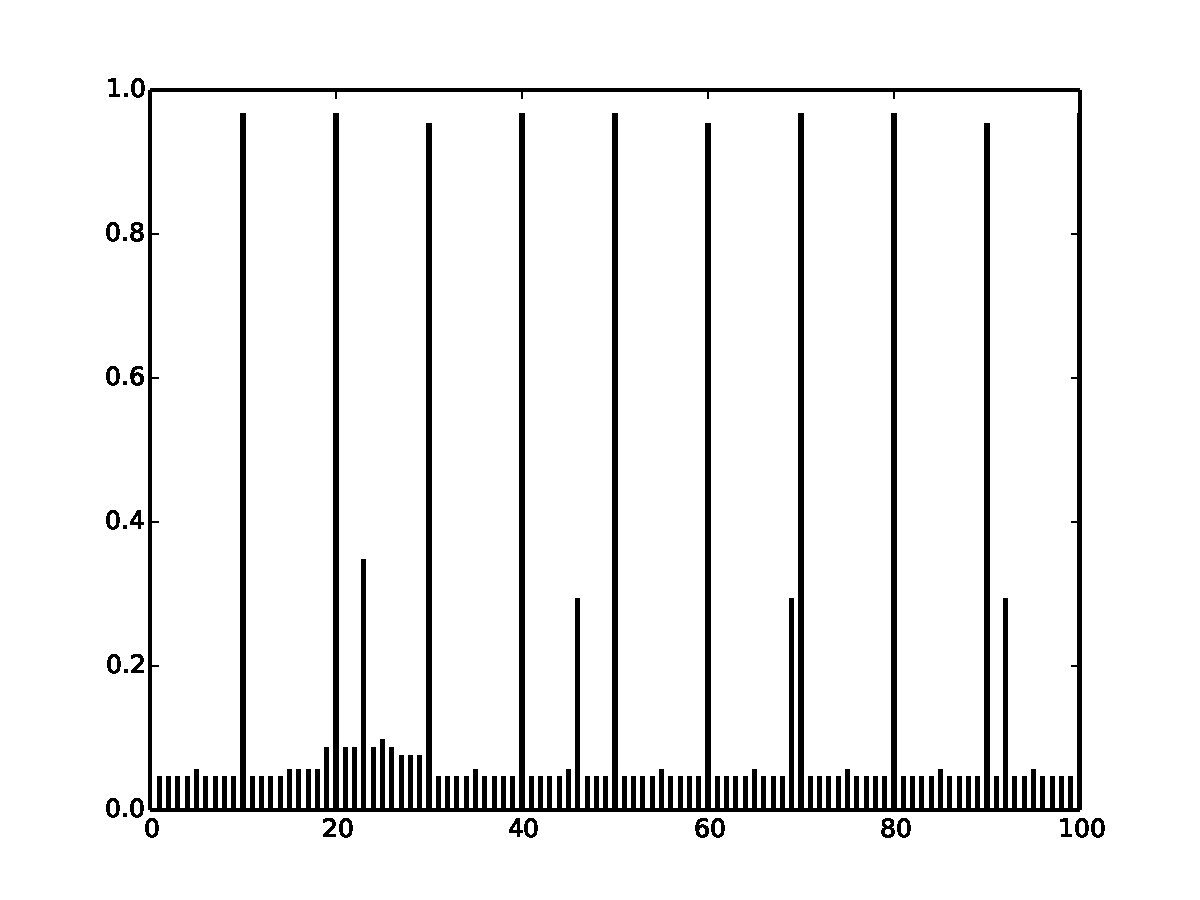
\includegraphics[scale=\Scale]{ng6080103023.pdf} &
	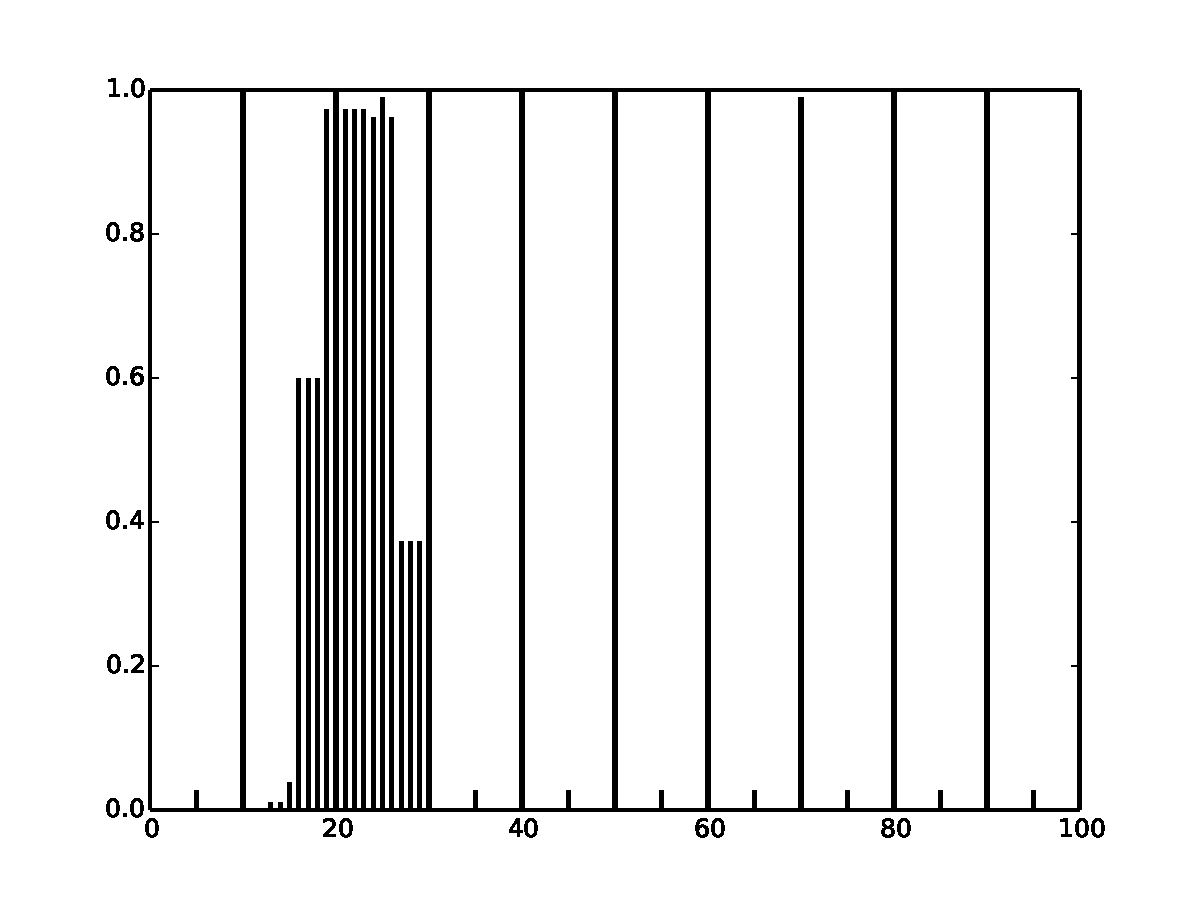
\includegraphics[scale=\Scale]{ng60801030232521.pdf}
	\end{tabular}
	\caption{Generalization probabilities in the numbers world, according to
	the model.}
	\label{numbersplot}
\end{figure*}

A clear size principle emerges with the change of 
grammar.\footnote{In this section, each finding comes uses
20000--30000 samples with $b=1.3$. The number of samples had
to be reduced to $20000$ sometimes because our implementation,
which memoizes formulas, tended to result in memory errors
with $30000$ samples on some imputs.} For
example, if the observed data tells the learner only that $60\in C$,
then the top hypothesis is that $C$ consists of multiples of 30:
the formula $f_{30}(x)$ is only true for three numbers, whereas
the formula $f_{10}(x)$, for instance, is true for ten numbers;
this gives $f_{30}(x)$ a boost over $f_{10}(x)$ in the posterior.

However, the size principle, a consequence of the likelihood,
 is offset by the prior's aversion to complicated formulae.
The formula $f_{30}(x)\wedge g_{60}(x)$ defines an even more
exclusive club of just one, but it is beat by $f_{30}(x)$ in
the posterior because its derivation has more steps.

The addition of evidence can push the posterior back in the direction
of more complicated formulae. For example, with the evidence that
$\{58, 59, 61, 62\} \subset C$, the
top three formulae are
\[ g_{63}(x)\quad g_{57}(x) \quad g_{63}(x)\wedge g_{57}(x). \]
The third formula here defines a narrower cluster of numbers.
If new evidence falls outside this hypothesis, the model adjusts
itself: told that $\{58, 59, 61, 62, 64, 65, 67, 68\} \subset C$,
the model chooses
\[ g_{63}(x)\quad \neg f_3(x)\wedge g_{63}(x) 
    \quad g_{63}(x)\wedge\neg f_3(x) \]
as its top three formulae.

Figure~\ref{numbersplot} further illustrates some of the same principles.
We did not gather human data, though it would be interesting to
see whether the model matches humans learning of compound rules.
On those input sets for which \citet{numbergame} provides human data,
our model does not track the human responses as well as the original model
does, but some of the qualitative effects are still present.


\section{A world of animals}

In this section we consider a world of 33~animals and 102~features
provided by \citet{kemp}, who give a graphical model that predicts
the tree structure of animal categories. A tree structure strongly
suggests a prior over concept hypotheses that favors concepts that
correspond to subtrees of the hierarchy. The size principle then
predicts that the most likely concept given several positive examples
is the smallest subtree containing them. Thus for poodles and
labrador retrievers the category is dogs; for
poodles, lions, and horses --- mammals; and for poodles, fish,
and roaches --- all animals.

In many cases we find that the concept grammar model does show
this smallest subtree effect.
(With the original grammar the model runs into the same problem
as it did with the number game, so again we use the grammar in 
figure~\ref{dnf2}.) Below are summaries
of the  model's generalizations (30000 samples each, $b=3$) 
on various inputs.

\begin{rdescription} % pos too
\item[Positive examples] Dog, Wolf 
\item[Likely formulae\footnotemark]
	\footnotetext{The smallest cut from the top
	of the list of the most likely formulae
	(in the posterior) that accounts for more than half 
	the probability mass of the top $\phi=10$ formulae. The formulae
	are listed in order of decreasing posterior
	probability.} howls; is a canine $\wedge$
	eats rodents
\item[Likely examples\footnotemark]
	\footnotetext{Those objects with generalization
	probability at least 0.5, in order of decreasing
	generalization probability.}
	Dog, Wolf
\item[Smallest subtree\footnotemark]
	\footnotetext{The animals in the smallest subtree 
	(of the tree in
	\citealt{kemp}) that contains 
	all of the positive examples.} (same)
\end{rdescription}

\begin{rdescription} % pos too
\item[Positive examples] Cat, Dog, Wolf
\item[Likely formulae] eats rodents
\item[Likely examples]
	Cat, Dog, Wolf, Eagle
\item[Smallest subtree] Cat, Dog, Wolf
\end{rdescription}

\begin{rdescription}
\item[Positive examples] Cat, Tiger, Wolf
\item[Likely formulae] has paws; digs holes
\item[Likely examples]
	Tiger, Lion, Cat, Dog, Wolf % pos adds Squirrel
\item[Smallest subtree]
	(same)
\end{rdescription}

\begin{rdescription}
\item[Positive examples] Chimp, Wolf, Rhino
\item[Likely formulae] has visible ears; has 4 legs; runs; has a nose
\item[Likely examples]
	Rhino, Chimp, Gorilla, Lion, Dog, Wolf, Horse, Camel, Giraffe,
	Tiger, Cat, Elephant, Mouse, Squirrel, Deer, Cow, Seal
\item[Smallest subtree]
	(same, except for Seal)
\item[Intended category] mammals
\end{rdescription}

\begin{rdescription}
\item[Positive examples] Camel, Cow, Elephant
\item[Likely formulae] has hooves
\item[Likely examples] Elephant, Rhino, Horse, Cow, Camel,
	Giraffe, Deer
\item[Smallest subtree] (same)
\end{rdescription}

\begin{rdescription}
\item[Positive examples] Ant, Bee
\item[Likely formulae] is an insect; $\neg$ has bones; $\neg$ has red blood;
	flies
\item[Likely examples]
	Bee, Butterfly, Ant, Cockroach
\item[Smallest subtree]
	(same)
\end{rdescription}


\begin{rdescription}
\item[Positive examples] Chicken, Eagle
\item[Likely formulae] is a bird, has a beak, has 2 legs
\item[Likely examples]
	Robin, Eagle, Chicken, Ostrich, Finch, Penguin
\item[Smallest subtree]
	(same, except for Penguin)
\item[Intended category] birds
\end{rdescription}


\begin{rdescription}
\item[Positive examples] Finch, Robin
\item[Likely formulae] sings; eats nuts
\item[Likely examples]
	Robin, Finch
\item[Smallest subtree]
	(same)
\item[Intended category] birds that can fly
\end{rdescription}

However, when the smallest subtree containing the positive examples
 is the entire of tree of animals, the model, ever faithful to the
size principle, tends to come up with categories that do not match
human intuitions:

\begin{rdescription}
\item[Positive examples] Salmon, Wolf
\item[Likely formulae] lives in cold climates; eats fish
\item[Likely examples]
	Wolf, Salmon, Dog, Seal, Penguin, Whale, Cat, Eagle, Dolphin,
	Tiger, Trout, Ant
\item[Smallest subtree]
	(all 33 animals)
\end{rdescription}

\begin{rdescription}
\item[Positive examples] Ant, Ostrich, Tiger
\item[Likely formulae] $\neg$ is brown; lives in hot climates;
	$\neg$ has a snout
\item[Likely examples]
	(23 animals)
	%Cockroach, Tiger, Ostrich, Ant, Lion, Elephant, Gorilla, Bee
	%Rhino, Penguin, Salmon, Cat, Camel, Mouse, Dolphin,
	%Alligator, Chimp, Whale, Trout, Butterfly, Wolf, Chicken,
	%Iguana
\item[Smallest subtree]  (all 33 animals)
	%Alligator, Ant, Bee, Butterfly, Camel, Cat,
	% Chicken, Chimp, Cockroach, \emph{Cow}, \emph{Deer}, \emph{Dog},
	% Dolphin, \emph{Eagle},
	% Elephant, Finch, \emph{Giraffe},
	% Gorilla, \emph{Horse}, Iguana, Lion, \emph{Mouse},
	% Ostrich, Penguin, Rhino, \emph{Robin},
	% Salmon, \emph{Seal}, \emph{Squirrel}, Tiger,
	% Trout, Whale, Wolf
\end{rdescription}

It's not easy to come up with a set that the model
generalizes to all 33~animals. 

\begin{rdescription}
\item[Positive examples] Bee, Giraffe, Penguin
\item[Likely formulae] travels in groups; $\neg$ is smart; is black
\item[Likely examples] (21 animals)
\item[Smallest subtree] (all 33 animals)
\end{rdescription}

\begin{rdescription}
\item[Positive examples] Bee, Giraffe, Penguin, Eagle
\item[Likely formulae] is soft; $\neg$ bites; $\neg$ digs holes
\item[Likely examples] (31 animals)
\item[Smallest subtree] (all 33 animals)
\end{rdescription}

\begin{rdescription}
\item[Positive examples] Bee, Giraffe, Penguin, Eagle, Ant
\item[Likely formulae] $\neg$ has a large brain; $\neg$ eats seeds;
	$\neg$ eats bugs; $\neg$ is a feline 
\item[Likely examples] (32 animals)
\item[Smallest subtree] (all 33 animals)
\end{rdescription}

Most of the formulae above only involve one feature, suggesting that
our compositional concept space is overkill. 
Here is a failed attempt
at getting the model to learn a compound rule:

\begin{rdescription}
\item[Positive examples] Robin, Finch, Chicken, Ant,
	 Bee, Butterfly, Cockroach
\item[Likely formulae] $\neg$ has teeth
\item[Likely examples] Cockroach, Robin, Chicken, Bee, Butterfly,
	Ant, Finch, Ostrich, Eagle
\item[Smallest subtree]
	the above, and Penguin, Salmon, Trout, Alligator, Iguana
\end{rdescription}

And a successful attempt:

\begin{rdescription}
\item[Positive examples] Salmon, Trout, Wolf, Dog
\item[Likely formulae] is a fish $\vee$ is a canine;
	 is a fish $\vee$ howls
\item[Likely examples]
	Dog, Wolf, Salmon, Trout
\item[Smallest subtree]
	(all 33 animals)
\end{rdescription}

Still, the full combinatorial power of the model is hardly engaged.

If we allowed the input to be lists of observations rather than
sets of objects, that is, if objects could be repeated in the input,
there would be more possible experiments. For example, the repeated
observation of, say, a cockroach, a salmon, and a dog as being
part of a category should eventually cause the model to 
posit a concept containing those three animals \emph{and nothing else},
no matter how convoluted the formula is.

\bibliography{report}

\end{document}

